\subsection{Reflexão das Linhas Superiores}

\begin{figure}[!htb]
    \centering
    \begin{subfigure}{0.45\textwidth}
        \centering
        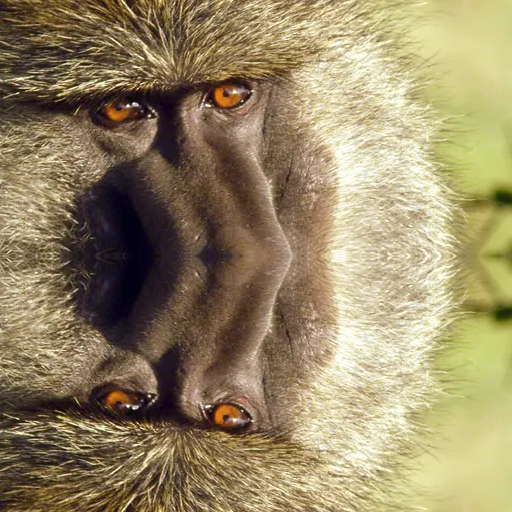
\includegraphics[width=6cm]{resultados/colorrefl.png}
        \caption{\texttt{imagens/color.png}}
    \end{subfigure}%
    \begin{subfigure}{0.45\textwidth}
        \centering
        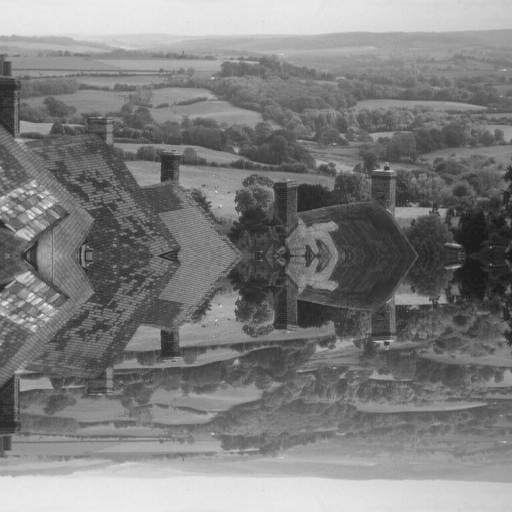
\includegraphics[width=6cm]{resultados/cityrefl.png}
        \caption{\texttt{imagens/city.png}}
    \end{subfigure}

    \caption{Linhas superiores refletidas.}
\end{figure}

\begin{listing}[htb]
    \caption{Comando \texttt{reflexao}}

    \begin{minted}{python}
        def reflexao_linhas(imagem):
            mid = len(image) // 2
            imagem[-mid:] = imagem[:mid][::-1]
            return imagem
    \end{minted}
\end{listing}
